\subsection{Discuss the coherent interaction between atoms and light using the Bloch vector formalism. Give an example for experiment which can be described using the Bloch vector.}


Vi kigger på et toniveausystem, hvor bølgefunktionen for dette system vil være
\begin{align} \label{eq:Q04_TotalBoelgefunktionTidsafhaengig}
    \Psi(\Vec{r},t) &= c_1\ket{1}\exp{-i\omega_1 t} + c_2\ket{2}\exp{-i\omega_2 t} \: ,
\end{align}
hvor $c_j = c_j(t)$ og $\omega_j = E_j/\hbar$ for $j = 1,\,2$.

Påvirkes dette toniveausystem nu af elektromagnetisk stråling (lys) fra et oscillerende elektrisk felt $\Vec{E} = \Vec{E}_0$ resulterer dette i perturbationen
\begin{align}
    H'(t) &= e\Vec{r} \cdot \Vec{E}_0 \cos(\omega t) \: .
\end{align}
Dette leder til et induceret dipolmoment ifølge \textsf{dipolapproksimationen}\footnote{Et atom kan approksimeres til at være en dipol. Dipolapproksimationen holder så længe, at lysets bølgelængde er større end atomet, $\lambda \gg a_0$.} Vi lader nu lyset være polariseret langs $x$-aksen, hvorved komponenten af dipolen langs denne akse vil være givet ved forventningsværdien
\begin{align} \label{eq:Q04_ElektronladningGangeInduceretDipolmoment}
    -eD_x(t) = -\bra{\Psi(t)}ex\ket{\Psi(t)} = -e\left(c_2^*c_1X_{21}\exp{i\omega_0 t} + c_1^*c_2Z_{12}\exp{-i\omega_0 t}\right) \: ,
\end{align}
hvor $\omega_0 = \omega_2 - \omega_1 = \Delta \omega$ og $X_{ij} = \bra{i}x\ket{j}$, idet der er gjort brug af bølgefunktionen fra \cref{eq:Q04_TotalBoelgefunktionTidsafhaengig}. Dipolmomentet giver en reel værdi, idet $X_{ij} = \bra{i}x\ket{j} \Rightarrow X_{21} = (X_{12})^*$, og at $X_{11} = X_{22} = 0$. For at beregne dipolmomentet $D_x(t)$ induceret af det elektriske felt, da bliver vi nødt til at kende $c_1^*c_2$ og $c_2^*c_1$, hvilke er elementer i \textsf{densitetsmatricen}
\begin{align} \label{eq:Q04_DensityMatrix}
    \ketbra{\psi}{\Psi} &=
        \begin{pmatrix}
            c_1 \\
            c_2
        \end{pmatrix}
        \begin{pmatrix}
            c_1^* & c_2^*
        \end{pmatrix}
    = \begin{pmatrix}
            \abs{c_1}^2 & c_1c_2^* \\
            c_2c_1^* & \abs{c_2}^2
        \end{pmatrix}
    = \begin{pmatrix}
            \rho_{11} & \rho_{12} \\
            \rho_{21} & \rho_{22} \\
        \end{pmatrix}
    \: .
\end{align}
Her beskriver diagonalelementerne ($|c_1|^2$ og $|c_2|^2$) populationerne i hhv. grundtilstanden og den exciterede tilstand, mens antidiagonalelementerne (eng. the off-diagonal elements) kaldes \textsf{kohærenser} (eng. coherences) og beskriver systemet ved drivfrekvensen (\cref{eq:Q04_ElektronladningGangeInduceretDipolmoment}).

Vi definerer nu to nye variable (for at fjerne den trivielle fase)
\begin{align}
    \widetilde{c}_1 &= c_1\exp{-\frac{i\delta t}{2}} \: , \\
    \widetilde{c}_2 &= c_2\exp{\frac{i\delta t}{2}} \: ,
\end{align}
hvor $\delta = \omega - \omega_0$ kaldes \textsf{detuningen}\footnote{Fordansket oversættelse af ''the detuning''.} (afvigelsen) af lysets frekvens fra atomets ræsonansfrekvens. Denne transformation ændrer ikke på populationerne, hvorfor
\begin{align}
    \widetilde{\rho}_{11} &= \rho_{11} \quad \text{og} \quad \widetilde{\rho}_22 = \rho_{22} \: ,
\end{align}
men kohærencerne ændres til
\begin{align}
    \widetilde{\rho}_{12} &= \rho_{12}\exp{-i\delta t} \quad \text{og} \quad \widetilde{\rho}_{21} = \rho_{21}\exp{i\delta t} = (\widetilde{\rho}_{12})^* \: .
\end{align}
Beskrevet ved disse nye variable bliver dipolmomentet
\begin{align}
    -eD_x(t) &= -eX_{12}\left\{u\cos(\omega t) - v\sin(\omega t)\right\} \: ,
\end{align}
hvor
\begin{align}
    u &= \widetilde{\rho}_{12} + \widetilde{\rho}_{21} \: , \\
    v &= -i\left(\widetilde{\rho}_{12} + \widetilde{\rho}_{21}\right) \: .
\end{align}
Dipolmomenter er derved nu blevet beskrevet i systemet, som roterer med vinkelfrekvens $\omega$.

Ved at differentiere de givne densitetsmatrixelemter kan man opnå de optiske Blochligninger (ikke inkluderet spontan emission):
\begin{align} \label{eq:Q04_OpticalBlochEquations}
    \frac{\text{d}}{\text{d}t}\rho_{11} &= i \frac{\Omega}{2}\left(\widetilde{\rho}_{21} - \widetilde{\rho}_{12}\right) \: , \\
    \frac{\text{d}}{\text{d}t}\rho_{22} &= i \frac{\Omega}{2}\left(\widetilde{\rho}_{12} - \widetilde{\rho}_{21}\right) \: , \\
    \frac{\text{d}}{\text{d}t}\widetilde{\rho}_{12} &= -i\delta\widetilde{\rho}_{12} + i \frac{\Omega}{2}\left(\rho_{22} - \rho_{11}\right) \: , \\
    \frac{\text{d}}{\text{d}t}\widetilde{\rho}_{21} &= i\delta\widetilde{\rho}_{21} + i \frac{\Omega}{2}\left(\rho_{11} - \rho_{22}\right) \: ,
\end{align}
hvor $\widetilde{\rho}_{12}$ og $\widetilde{\rho}_{21}$ er defineret i det roterende system, $\widetilde{\rho}_{11} = \rho_{11}$ og $\widetilde{\rho}_{22} = \rho_{22}$, $\Omega$ er Rabifrekvensen og $\delta = \omega - \omega_0$ er detuningen.

Beskrives disse optiske Blochligninger som funktion af $u$, $v$ og $w = \rho_{11} - \rho_{22}$, da fås
\begin{align}
    \Dot{u} &= \delta v \: , \label{eq:Q04_DotU} \\
    \Dot{v} &= -\delta u + \Omega w \: , \label{eq:Q04_DotV} \\
    \Dot{w} &= -\Omega v \: . \label{eq:Q04_DotW}
\end{align}
Ved at definere \textsf{Blochvektoren} som $\Vec{R} = u\Hat{e}_1 + v\Hat{e}_2 + w\Hat{e}_3$ kan \cref{eq:Q04_DotU,eq:Q04_DotV,eq:Q04_DotW} skrives som
\begin{align} \label{eq:Q04_DotBlochVector}
    \Dot{\Vec{R}} &= \Vec{R} \cross \Vec{W} = \Vec{R} \cross \left(\Omega\Hat{e}_1 + \delta\Hat{e}_3\right) \: .
\end{align}
Her er $\Omega$ Rabifrekveensen, hvilket er den frekvens, som populationen drives med, og $\delta = \omega - \omega_0$ er detuningen.

Af \cref{eq:Q04_DotBlochVector} følger nogle vigtige egenskaber:
\begin{itemize}
    \item Grundet krydsproduktet må $\Dot{\Vec{R}} \perp \Vec{R}$, hvilket giver, at $|\Vec{R}|^2 = \text{konstant}$, og det kan vises, at $|\Vec{R}|^2 = 1$. Blochvektoren beskriver altså positionen af et punkt på en sfære med radius $1$, hvilket kaldes Blochsfæren.
    \item Grundet krydsproduktet må $\Dot{\Vec{R}} \perp \Vec{W}$, hvorfor $\Dot{\Vec{R}} \cdot \Vec{W} = 0$, så $\Vec{R} \cdot \Vec{W} = RW\cos(\theta) = \text{konstant}$. Sker der excitation med en konstant Rabifrekvens og detuning vil $W$ være konstant, og siden $R$ er fast, så vil Blochvektoren bevæge sig rundt om Blochsfæren i en cirkelbevægelse med konstant vinkel $\theta$.
\end{itemize}

\begin{figure}[!h]
    \centering
    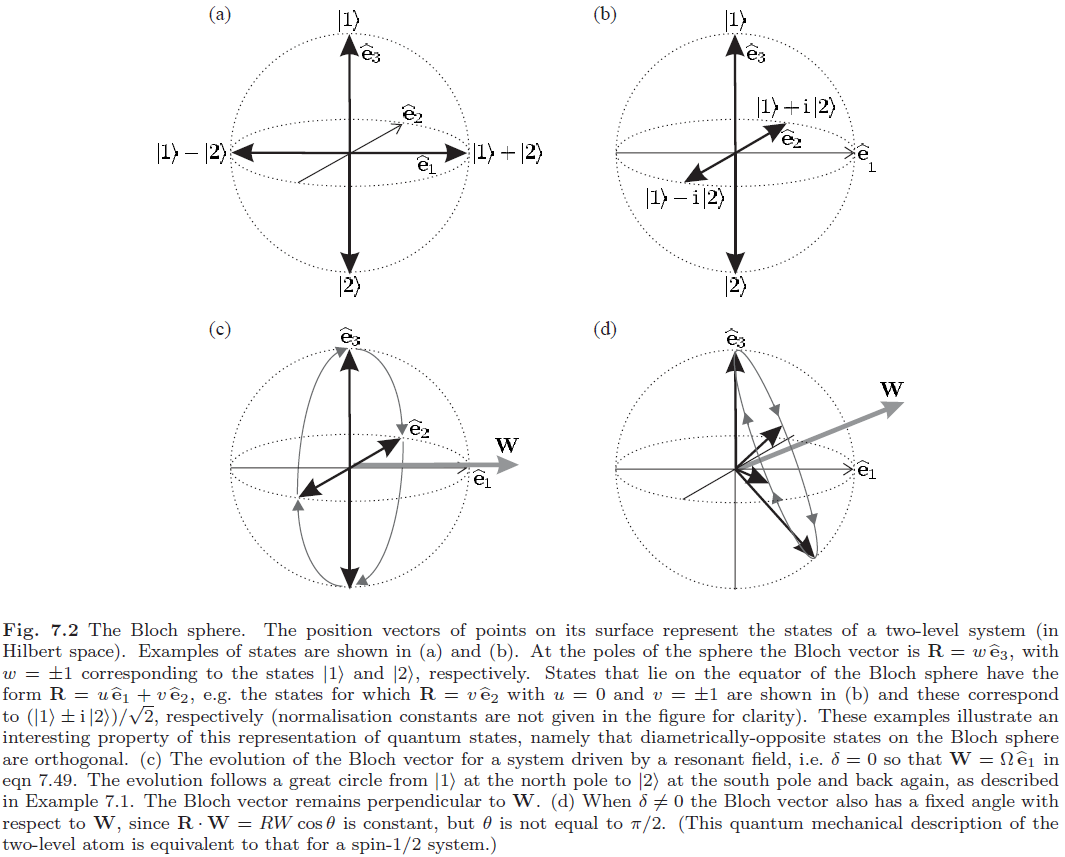
\includegraphics[width=\textwidth]{Q04/images/BlochSphere.PNG}
    \caption{}
    \label{fig:Q04_BlochSphere}
\end{figure}


\paragraph{Ekperiment beskrivet ved Blochvektorformalismen:} \ldots Atomuret